\documentclass[12pt,a4paper]{article}
\usepackage[utf8]{inputenc}
\usepackage[english,russian]{babel}
\usepackage{amssymb,amsfonts,amsmath,cite,enumerate,float,indentfirst}
\usepackage{graphicx}
\usepackage{geometry}
\usepackage{systeme}
\usepackage{amsmath}
\usepackage[bottom]{footmisc}
\usepackage{hyperref}
\usepackage{url}

\hypersetup{
	colorlinks,
	citecolor=black,
	filecolor=black,
	linkcolor=black,
	urlcolor=black
}
\geometry{left=2cm}
\geometry{right=1.5cm}
\geometry{top=2cm}
\geometry{bottom=2cm}


\begin{document}
	\begin{titlepage}
		\begin{center}		
			\vfill	
			Санкт-Петербургский политехнический университет \\
			Петра Великого\\
			\vskip 1cm
			Высшая школа прикладной математики и вычислительной физики \\
			Кафедра «Прикладная математика и информатика»
			\vfill
			\textbf{Отчёт\\
				по лабораторной работе №2\\
				по дисциплине\\
				«Интервальный анализ»\\}
			\vfill
		\end{center}
		\vfill
		\hfill
		\begin{minipage}{0.4\textwidth}
			Выполнил студент:\\
			Лапотников Павел Вадимович\\
			группа: 5030102/90201\\
		\end{minipage}
		\vfill
		\hfill 
		\begin{minipage}{0.4\textwidth}
			Проверил:\\
			к.ф.-м.н., доцент\\
			Баженов Александр Николаевич\
		\end{minipage}
		\vfill
		\hfill 
		\begin{center}
			Санкт-Петербург\\2022 г.
		\end{center}
	\end{titlepage}
	
	\tableofcontents
	\listoffigures
	\pagebreak
    	
    	
    \section{Постановка задачи}
        Дана ИСЛАУ 
        \begin{equation}\label{islau_initial}
            \begin{cases}
            a\cdot x_1+b\cdot x_2=c\\
            1 \cdot x_1 - k\cdot x_2=0\\
            d\cdot x_1 + 0=e\\
            \end{cases}
        \end{equation}
        где $a, \: b, \: c, \: k, \: d, \: e$ - положительные интервалы
        
        Для нее необходимо провести вычисления и привести иллюстрации:
        \begin{itemize}
            \item Максимума распознающего функционала
            \item Достижения разрешимости ИСЛАУ за счет коррекции правой части
            \item Достижения разрешимости ИСЛАУ за счет коррекции матрицы в целом
            \item Достижения разрешимости ИСЛАУ за счет коррекции матрицы построчно
            \item Оценок вариабельности решения
        \end{itemize}
    
    \section{Теория}
        \subsection{Распознающий функционал}
            Выражения для распознающего функционала 
            \begin{equation*}
                \mathrm{Tol}(x)=\mathrm{Tol}(x,\mbf{A},\mbf{b})=\min_{1\leq i\leq m}\left\{\text{rad}{\mbf{b}_i}-\left|\text{mid}{\mbf{b}_i}-\sum_{j=1}^n \mbf{a}_{ij}x_j\right|\right\}
            \end{equation*}
            \begin{equation*}
                x\in\Xi_{\mathrm{tol}}\Leftrightarrow\mathrm{Tol}(x)\geq0
            \end{equation*}
            $\mathrm{Tol}(x)$ - достигает конечного максимума на всем $\mbb{R}^n$. С помощью максимума данного функционала можно судить о пустоте допускового множества решений ИСЛАУ. Если $\max\limits_{x\in\mbb{R}^n}\mathrm{Tol}(x)\geq0$, то допусковое множество не пусто, иначе $\Xi_{\mathrm{tol}}=\varnothing$
        
        
        \subsection{Достижение разрешимости}
        
            \subsubsection{Достижение разрешимости ИСЛАУ за счет коррекции матрицы}
                Идея метода заключается в модификации исходной матрицы ИСЛАУ. Для метода, предложенного в лекциях, нужно выполнения свойства о невырожденности интервалов компонент правой части ИСЛАУ. Так как исходная задача (\ref{islau_initial}) не удовлетворяет этому условию, в качестве достижения разрешимости ИСЛАУ за счет коррекции матрицы был взять иттерационный метод, на каждой иттерации которого уменьшается вдвое радиус интервалов матрицы, пока система не станет разрешмой или разница между границами интервала не станет меньше изначально заданного $\varepsilon$
        
            \subsubsection{Достижение разрешимости ИСЛАУ за счет коррекции правой части}
                Наиболее простой способ достижения разрешимости ИСЛАУ — ослабление
                ограничения в правой части ИСЛАУ. Эта операция увеличивает значение $\mathrm{Tol}(x)$ и позволяет достичь разрешимости за счет ослабления требований к точности решения. Для этого к каждой компоненте правой части ИСЛАУ добавим величины $K\cdot\nu_i\cdot[-1;1]$, где $i$ - номер компоненты, $\nu_i$ - вес, задающий относительное расширение $i$-й компоненты, $K$ - общий коэффициент расширения вектора $\mbf{b}$.
                Примем $\nu_i=1\;\forall i=\overline{1,3}$. Подберем $K$ таким образом, чтобы выполнялось $ K +\max\limits_{x\in\mbb{R}^n}\mathrm{Tol}(x)\geq0$
            
            
            
            
        \subsection{Оценки вариабельности решения}
            Для оценки вариабельности решений будем использовать абсолютную(ive) и относительную(rve) оценки:
            $$\mathrm{ive}(\mbf{A},\mbf{b})=\min\limits_{A\in\mbf{A}}\mathrm{cond}\:A\cdot||\mathrm{argmax}\:\mathrm{Tol}(x)||\frac{\max\limits_{x\in\mbb{R}^n}\mathrm{Tol}(x)}{||\mbf{b}||}$$
            $$\mathrm{rve}(\mbf{A},\mbf{b})=\min\limits_{A\in\mbf{A}}\mathrm{cond}\:A\cdot\max\limits_{x\in\mbb{R}^n}\mathrm{Tol}(x)$$
            
    \section{Реализация}
        Лабораторная работа выполнена с помощью встроенных средств языка программирования Python с использованием библиотек matplotlib, intvalpy, numpy в среде разработки Jupyter Notebook. 
        
    \section{Результаты}
        \subsection{Исходная ИСЛАУ}
        Рассмотрим следующую ИСЛАУ
        \begin{equation}\label{islau}
            \begin{cases}
            [0,\:2]\cdot x_1+[1,\:3]\cdot x_2=[3,\:7]\\
            x_1 - [-4,\:-2]\cdot x_2=[-0.5,\:0.5]\\
            [0.75,\:1.25]\cdot x_1=[3,\:5]\\
            [0.75,\:1.25]\cdot x_2=[0,\:2]\\
            \end{cases}
        \end{equation}
    
    
    Изначальная ИСЛАУ имеет пустое допусковое множество - максимум распознающего функционала в точке $(2.57,1.22)$ равен - -1.79. (Пометим звездочкой)
    \begin{figure}[H]
        \centering
        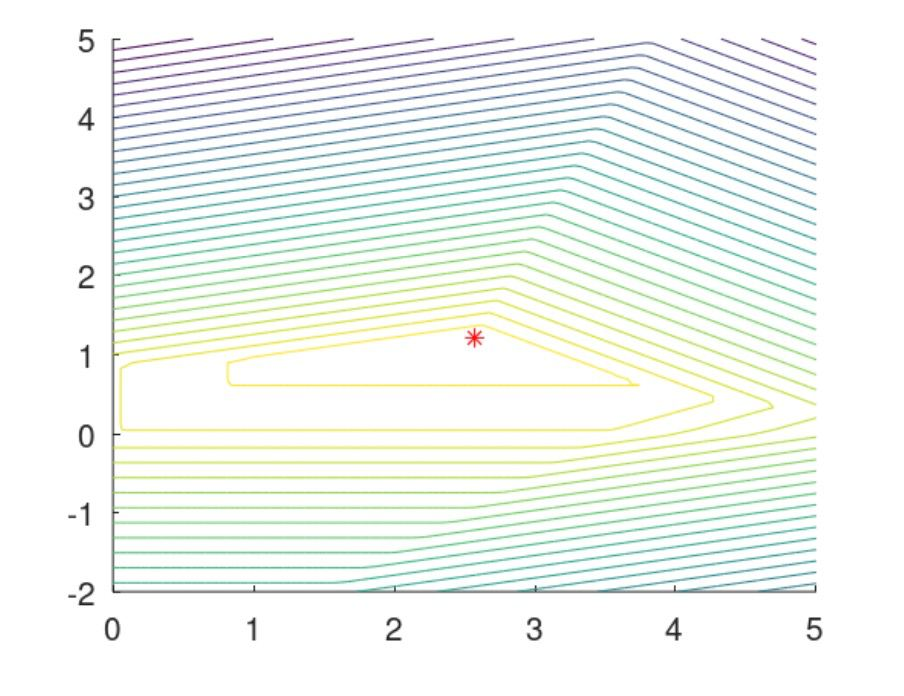
\includegraphics[width=16cm]{max_tol.png}
        \caption{График $\mathrm{Tol}(x,\mbf{A},\mbf{b})$}
        \label{fig:origtol}
    \end{figure}
    
    \subsection{Коррекция правой части}
    Заменим правую часть ИСЛАУ по описанной выше схеме. После коррекции максимум распознающего функционала стал равен $0.89$ в точке $(2.57,1.21)$.
    Вектор столбца
     $$
        \mathrm{b'} = ([0.32, 9.67],[−3.17, 3.17],[0.321,7.67],[−2.67, 4.67])
    $$
    \begin{figure}[H]
        \centering
        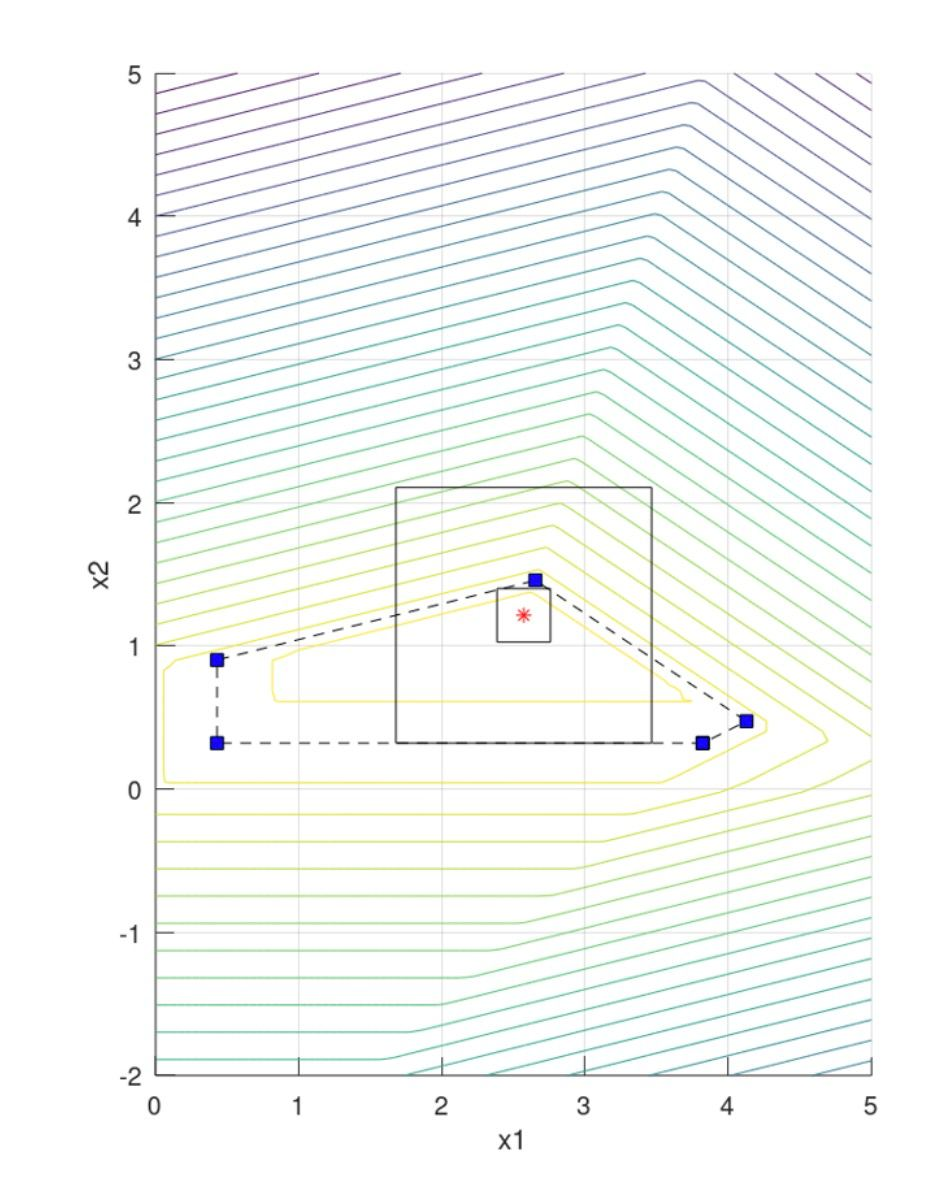
\includegraphics[width=16cm]{tol_right.png}
        \caption{$\mathrm{Tol}(x,\mbf{A}, \hat{\mbf{b}})$ для ИСЛАУ с правленной правой частью}
        \label{fig:btol}
    \end{figure}
    
    После коррекции правой части имеем следующие показатели ive и rve.
    $$
        \mathrm{ive}\:(\mbf{A}, \hat{\mbf{b}})\approx0.18
    $$
    
    $$
        \mathrm{rve}\:(\mbf{A}, \hat{\mbf{b}})\approx0.89
    $$
    На графике изображены квадратные брусы
с центром в точке максимума и радиусом ive и rve
    
    \subsection{Общая коррекция матрицы}
    
    После общей коррекции матрицы имеем максимум в точке $(3.52,1.12)$ - 0.34
    $$
        \mathrm{ive}\:(\mbf{A}, \hat{\mbf{b}})\approx-0.28
    $$
    
    $$
        \mathrm{rve}\:(\mbf{A}, \hat{\mbf{b}})\approx0.67
    $$ 
    \begin{figure}[H]
        \centering
        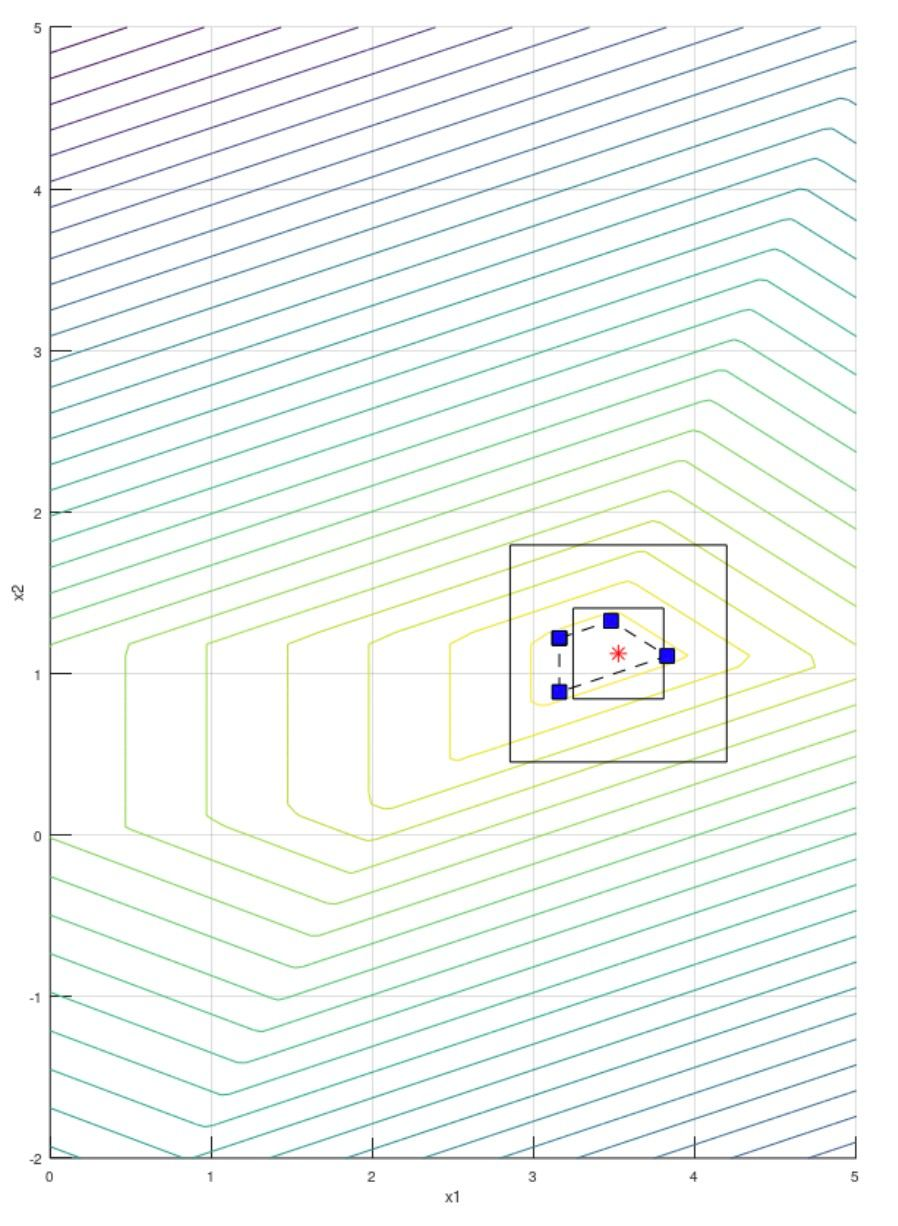
\includegraphics[height=16cm]{tol_left.png}
        \caption{$\Xi_{\mathrm{tol}}$ для ИСЛАУ с исправленной матрицей в целом}
        \label{fig:changeAGeneral}
    \end{figure}

    Матрица
    $$
    A' = \begin{pmatrix}
    [0.75, 1.25] & 2 \\
    1 & 3 \\
    [0.95, 1.05] & 0 \\
    0 & [0.75, 1.25]
    \end{pmatrix}
    $$
    
    \subsection{Коррекция матрицы построчно}
        \subsubsection{Первая строка}
            ИСЛАУ за счет коррекции первой строки имеет максимум распознающего функционала в точке $(3.23, 1.08)$
            \begin{figure}[H]
                \centering
                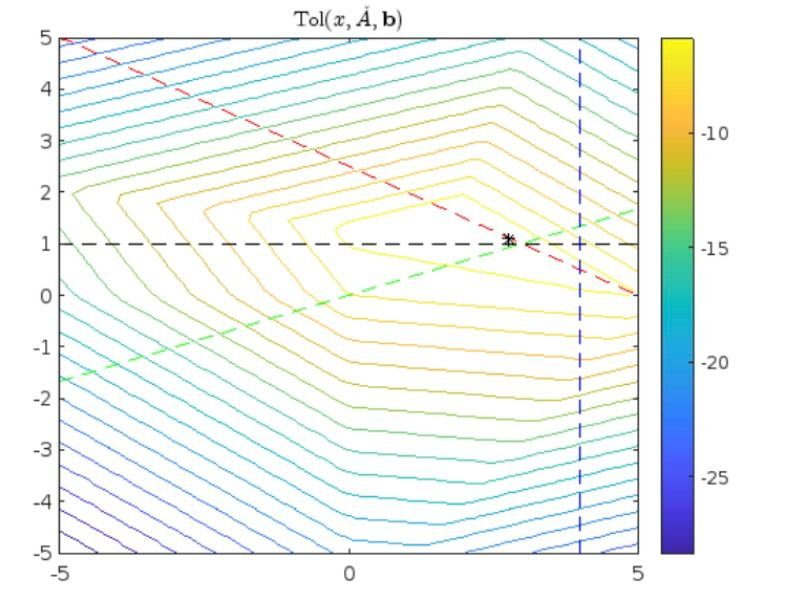
\includegraphics[width=16cm]{tol_first.png}
                \caption{$\mathrm{Tol}(x,\mbf{A}, \hat{\mbf{b}})$ для ИСЛАУ с исправленной первой строкой матрицы}
                \label{fig:aiverve}
            \end{figure}
            
        \subsubsection{Вторая строка}
            В результате коррекции второй строки матрицы имеет максимум распознающего функционала в точке $(2.17,1.42)$
            \begin{figure}[H]
                \centering
                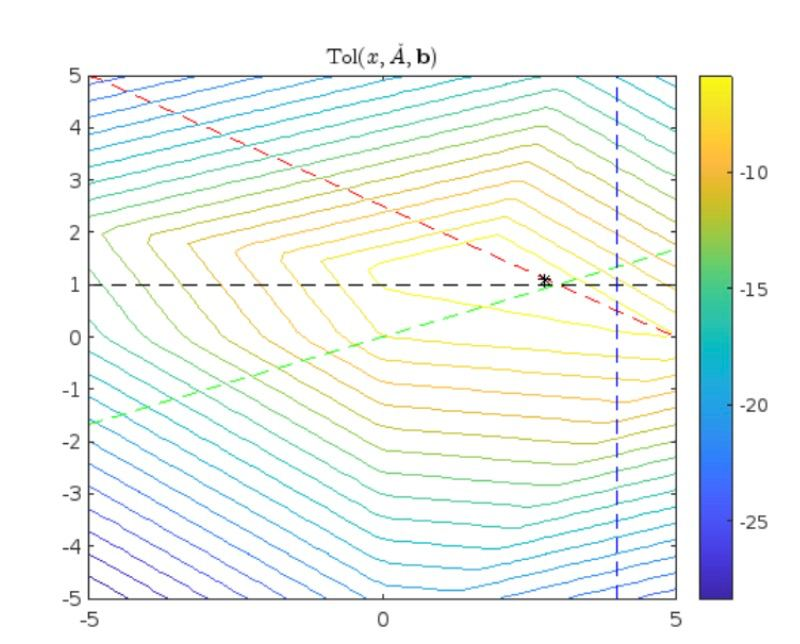
\includegraphics[width=16cm]{tol_second.png}
                \caption{$\mathrm{Tol}(x,\mbf{A}, \hat{\mbf{b}})$ для ИСЛАУ с исправленной второй строкой матрицы}
                \label{fig:aiverve}
            \end{figure}
            
        \subsubsection{Третья строка}
            В результате коррекции третьей строки матрицы, ИСЛАУ также не стала разрешимой. Максимум распознающего функционала в точке $(2.57, 1.21)$
            \begin{figure}[H]
                \centering
                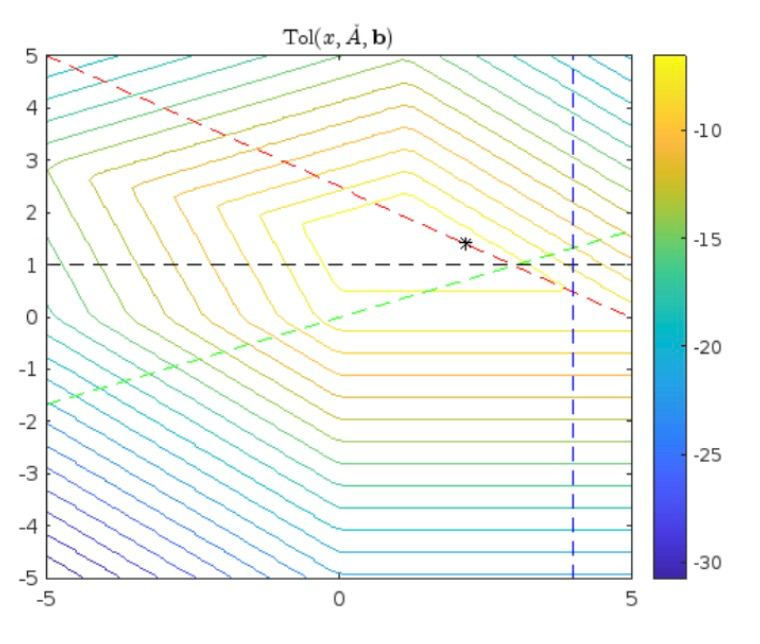
\includegraphics[width=16cm]{tol_third.png}
                \caption{$\mathrm{Tol}(x,\mbf{A}, \hat{\mbf{b}})$ для ИСЛАУ с исправленной третьей строкой матрицы}
                \label{fig:aiverve}
            \end{figure}
        \subsubsection{Четвертая строка}
            В результате коррекции четвертой строки матрицы, ИСЛАУ также не стала разрешимой. Максимум распознающего функционала в точке $(2.57, 1.21)$ 
            \begin{figure}[H]
                \centering
                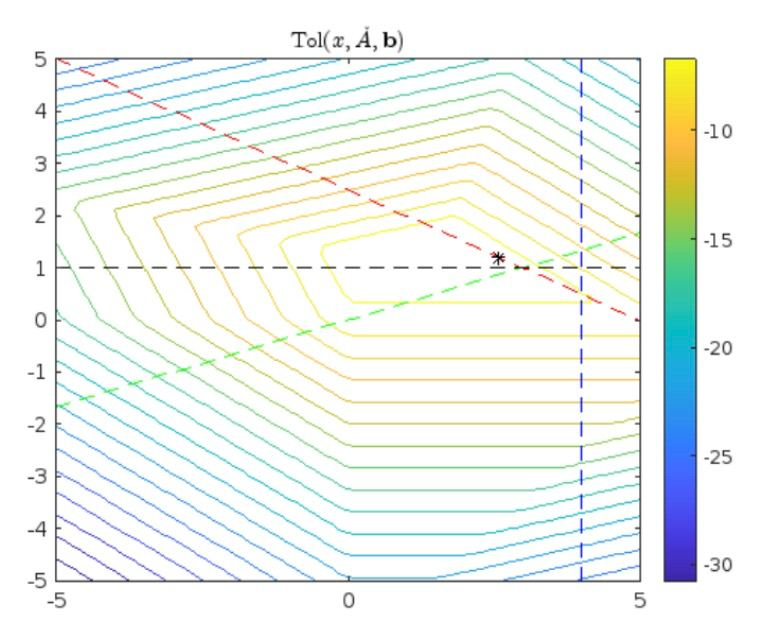
\includegraphics[width=16cm]{tol_fourth.png}
                \caption{$\mathrm{Tol}(x,\mbf{A}, \hat{\mbf{b}})$ для ИСЛАУ с исправленной четвертой строкой матрицы}
                \label{fig:aiverve}
            \end{figure}
        
    \section{Обсуждение}
        \begin{enumerate}
            \item Оценки вариабльности меньше при коррекции матрицы, при этом брусы, соответствующие оценкам вариабельности, хорошо оценили допусковое множество
итоговой ИСЛАУ
            \item Коррекция матрицы ИСЛАУ меняет форму распознающего функционала во
всех рассмотренных преобразованиях

            \item Во всех случаях исправления максимум распознавающего функционала располагается на прямой соответствующей медиане.
            
            \item При корректировки третьей строки можно наблюдать смещение центра максимума и при увеличении параметра, начиная с e = 0.2, положение максимума не
изменяется
            
            
        \end{enumerate}

    \section{Приложение}
        Код программы на GitHub Url https://github.com/lpvmak/interval
        
\end{document}
